% Options for packages loaded elsewhere
\PassOptionsToPackage{unicode}{hyperref}
\PassOptionsToPackage{hyphens}{url}
\PassOptionsToPackage{dvipsnames,svgnames,x11names}{xcolor}
%
\documentclass[
  letterpaper,
  DIV=11,
  numbers=noendperiod]{scrartcl}

\usepackage{amsmath,amssymb}
\usepackage{iftex}
\ifPDFTeX
  \usepackage[T1]{fontenc}
  \usepackage[utf8]{inputenc}
  \usepackage{textcomp} % provide euro and other symbols
\else % if luatex or xetex
  \usepackage{unicode-math}
  \defaultfontfeatures{Scale=MatchLowercase}
  \defaultfontfeatures[\rmfamily]{Ligatures=TeX,Scale=1}
\fi
\usepackage{lmodern}
\ifPDFTeX\else  
    % xetex/luatex font selection
\fi
% Use upquote if available, for straight quotes in verbatim environments
\IfFileExists{upquote.sty}{\usepackage{upquote}}{}
\IfFileExists{microtype.sty}{% use microtype if available
  \usepackage[]{microtype}
  \UseMicrotypeSet[protrusion]{basicmath} % disable protrusion for tt fonts
}{}
\makeatletter
\@ifundefined{KOMAClassName}{% if non-KOMA class
  \IfFileExists{parskip.sty}{%
    \usepackage{parskip}
  }{% else
    \setlength{\parindent}{0pt}
    \setlength{\parskip}{6pt plus 2pt minus 1pt}}
}{% if KOMA class
  \KOMAoptions{parskip=half}}
\makeatother
\usepackage{xcolor}
\usepackage[lmargin=30mm,rmargin=30mm]{geometry}
\setlength{\emergencystretch}{3em} % prevent overfull lines
\setcounter{secnumdepth}{-\maxdimen} % remove section numbering
% Make \paragraph and \subparagraph free-standing
\ifx\paragraph\undefined\else
  \let\oldparagraph\paragraph
  \renewcommand{\paragraph}[1]{\oldparagraph{#1}\mbox{}}
\fi
\ifx\subparagraph\undefined\else
  \let\oldsubparagraph\subparagraph
  \renewcommand{\subparagraph}[1]{\oldsubparagraph{#1}\mbox{}}
\fi


\providecommand{\tightlist}{%
  \setlength{\itemsep}{0pt}\setlength{\parskip}{0pt}}\usepackage{longtable,booktabs,array}
\usepackage{calc} % for calculating minipage widths
% Correct order of tables after \paragraph or \subparagraph
\usepackage{etoolbox}
\makeatletter
\patchcmd\longtable{\par}{\if@noskipsec\mbox{}\fi\par}{}{}
\makeatother
% Allow footnotes in longtable head/foot
\IfFileExists{footnotehyper.sty}{\usepackage{footnotehyper}}{\usepackage{footnote}}
\makesavenoteenv{longtable}
\usepackage{graphicx}
\makeatletter
\def\maxwidth{\ifdim\Gin@nat@width>\linewidth\linewidth\else\Gin@nat@width\fi}
\def\maxheight{\ifdim\Gin@nat@height>\textheight\textheight\else\Gin@nat@height\fi}
\makeatother
% Scale images if necessary, so that they will not overflow the page
% margins by default, and it is still possible to overwrite the defaults
% using explicit options in \includegraphics[width, height, ...]{}
\setkeys{Gin}{width=\maxwidth,height=\maxheight,keepaspectratio}
% Set default figure placement to htbp
\makeatletter
\def\fps@figure{htbp}
\makeatother

\KOMAoption{captions}{tablesignature}
\makeatletter
\@ifpackageloaded{caption}{}{\usepackage{caption}}
\AtBeginDocument{%
\ifdefined\contentsname
  \renewcommand*\contentsname{Table of contents}
\else
  \newcommand\contentsname{Table of contents}
\fi
\ifdefined\listfigurename
  \renewcommand*\listfigurename{List of Figures}
\else
  \newcommand\listfigurename{List of Figures}
\fi
\ifdefined\listtablename
  \renewcommand*\listtablename{List of Tables}
\else
  \newcommand\listtablename{List of Tables}
\fi
\ifdefined\figurename
  \renewcommand*\figurename{Figure}
\else
  \newcommand\figurename{Figure}
\fi
\ifdefined\tablename
  \renewcommand*\tablename{Table}
\else
  \newcommand\tablename{Table}
\fi
}
\@ifpackageloaded{float}{}{\usepackage{float}}
\floatstyle{ruled}
\@ifundefined{c@chapter}{\newfloat{codelisting}{h}{lop}}{\newfloat{codelisting}{h}{lop}[chapter]}
\floatname{codelisting}{Listing}
\newcommand*\listoflistings{\listof{codelisting}{List of Listings}}
\makeatother
\makeatletter
\makeatother
\makeatletter
\@ifpackageloaded{caption}{}{\usepackage{caption}}
\@ifpackageloaded{subcaption}{}{\usepackage{subcaption}}
\makeatother
\ifLuaTeX
  \usepackage{selnolig}  % disable illegal ligatures
\fi
\usepackage{bookmark}

\IfFileExists{xurl.sty}{\usepackage{xurl}}{} % add URL line breaks if available
\urlstyle{same} % disable monospaced font for URLs
\hypersetup{
  pdftitle={Run 001 Summary},
  pdfauthor={Pranav Kumar Mishra},
  colorlinks=true,
  linkcolor={blue},
  filecolor={Maroon},
  citecolor={Blue},
  urlcolor={Blue},
  pdfcreator={LaTeX via pandoc}}

\title{Run 001 Summary}
\usepackage{etoolbox}
\makeatletter
\providecommand{\subtitle}[1]{% add subtitle to \maketitle
  \apptocmd{\@title}{\par {\large #1 \par}}{}{}
}
\makeatother
\subtitle{An analysis of the MBSA-QIP Dataset}
\author{Pranav Kumar Mishra}
\date{Wednesday, May 29, 2024}

\begin{document}
\maketitle

\renewcommand*\contentsname{Table of contents}
{
\hypersetup{linkcolor=}
\setcounter{tocdepth}{3}
\tableofcontents
}
\section{Run 001 Summary}\label{run-001-summary}

Generated: 2024-05-29

\subsection{Run Parameters:}\label{run-parameters}

\begin{itemize}
\tightlist
\item
  CPT Codes: \texttt{{[}\textquotesingle{}43644\textquotesingle{}{]}}
\item
  Year Start: \texttt{2021}
\item
  Year Stop: \texttt{2022}
\end{itemize}

\subsection{Dataset}\label{dataset}

\begin{itemize}
\tightlist
\item
  Subjects: \texttt{269,926}
\item
  \href{data/analysis/bariatric/runs/run_001/tables/Run001_main_dataset.parquet}{Main
  Dataset Parquet}
\item
  \href{data/analysis/bariatric/runs/run_001/tables/Run001_demo_selected.csv}{Demo
  CSV - Random 20 Subjects}
\end{itemize}

\subsection{Figures}\label{figures}

\begin{figure}[H]

{\centering 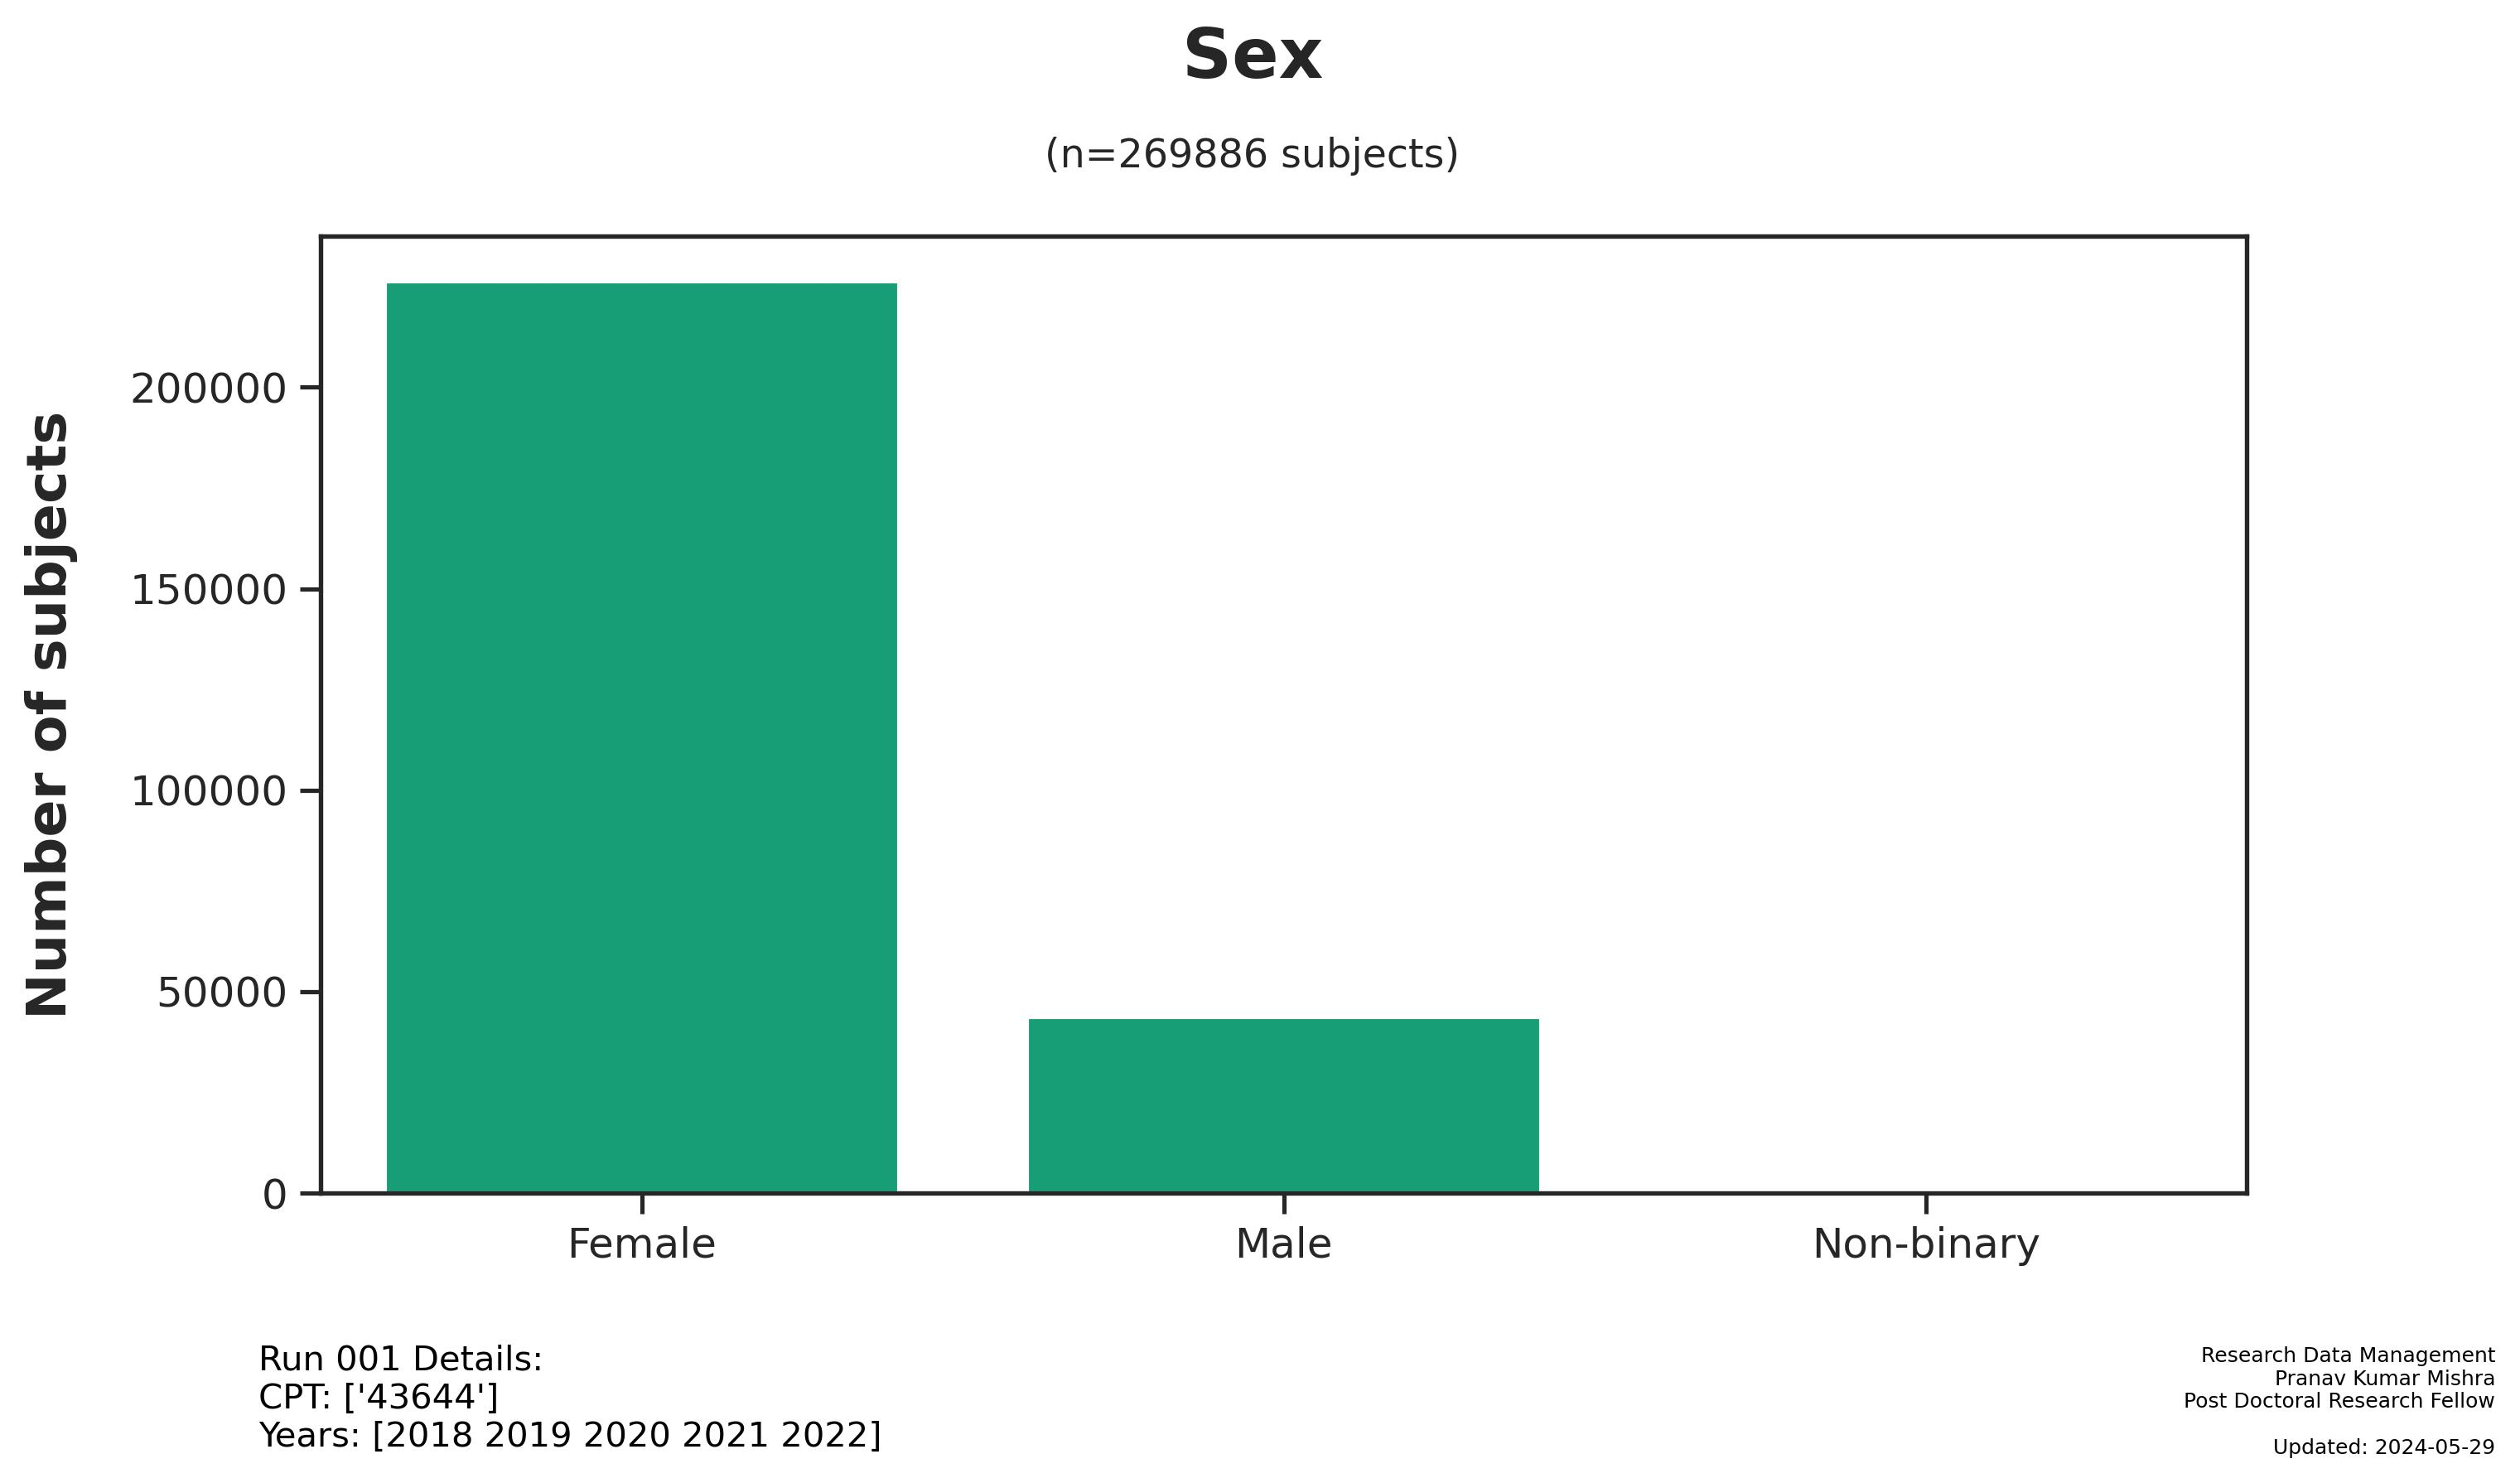
\includegraphics{figures/demographics/Run001_Demographics-Donor_Sex.jpg}

}

\caption{Run001\_Demographics-Donor\_Sex.jpg}

\end{figure}%%
\begin{figure}[H]

{\centering 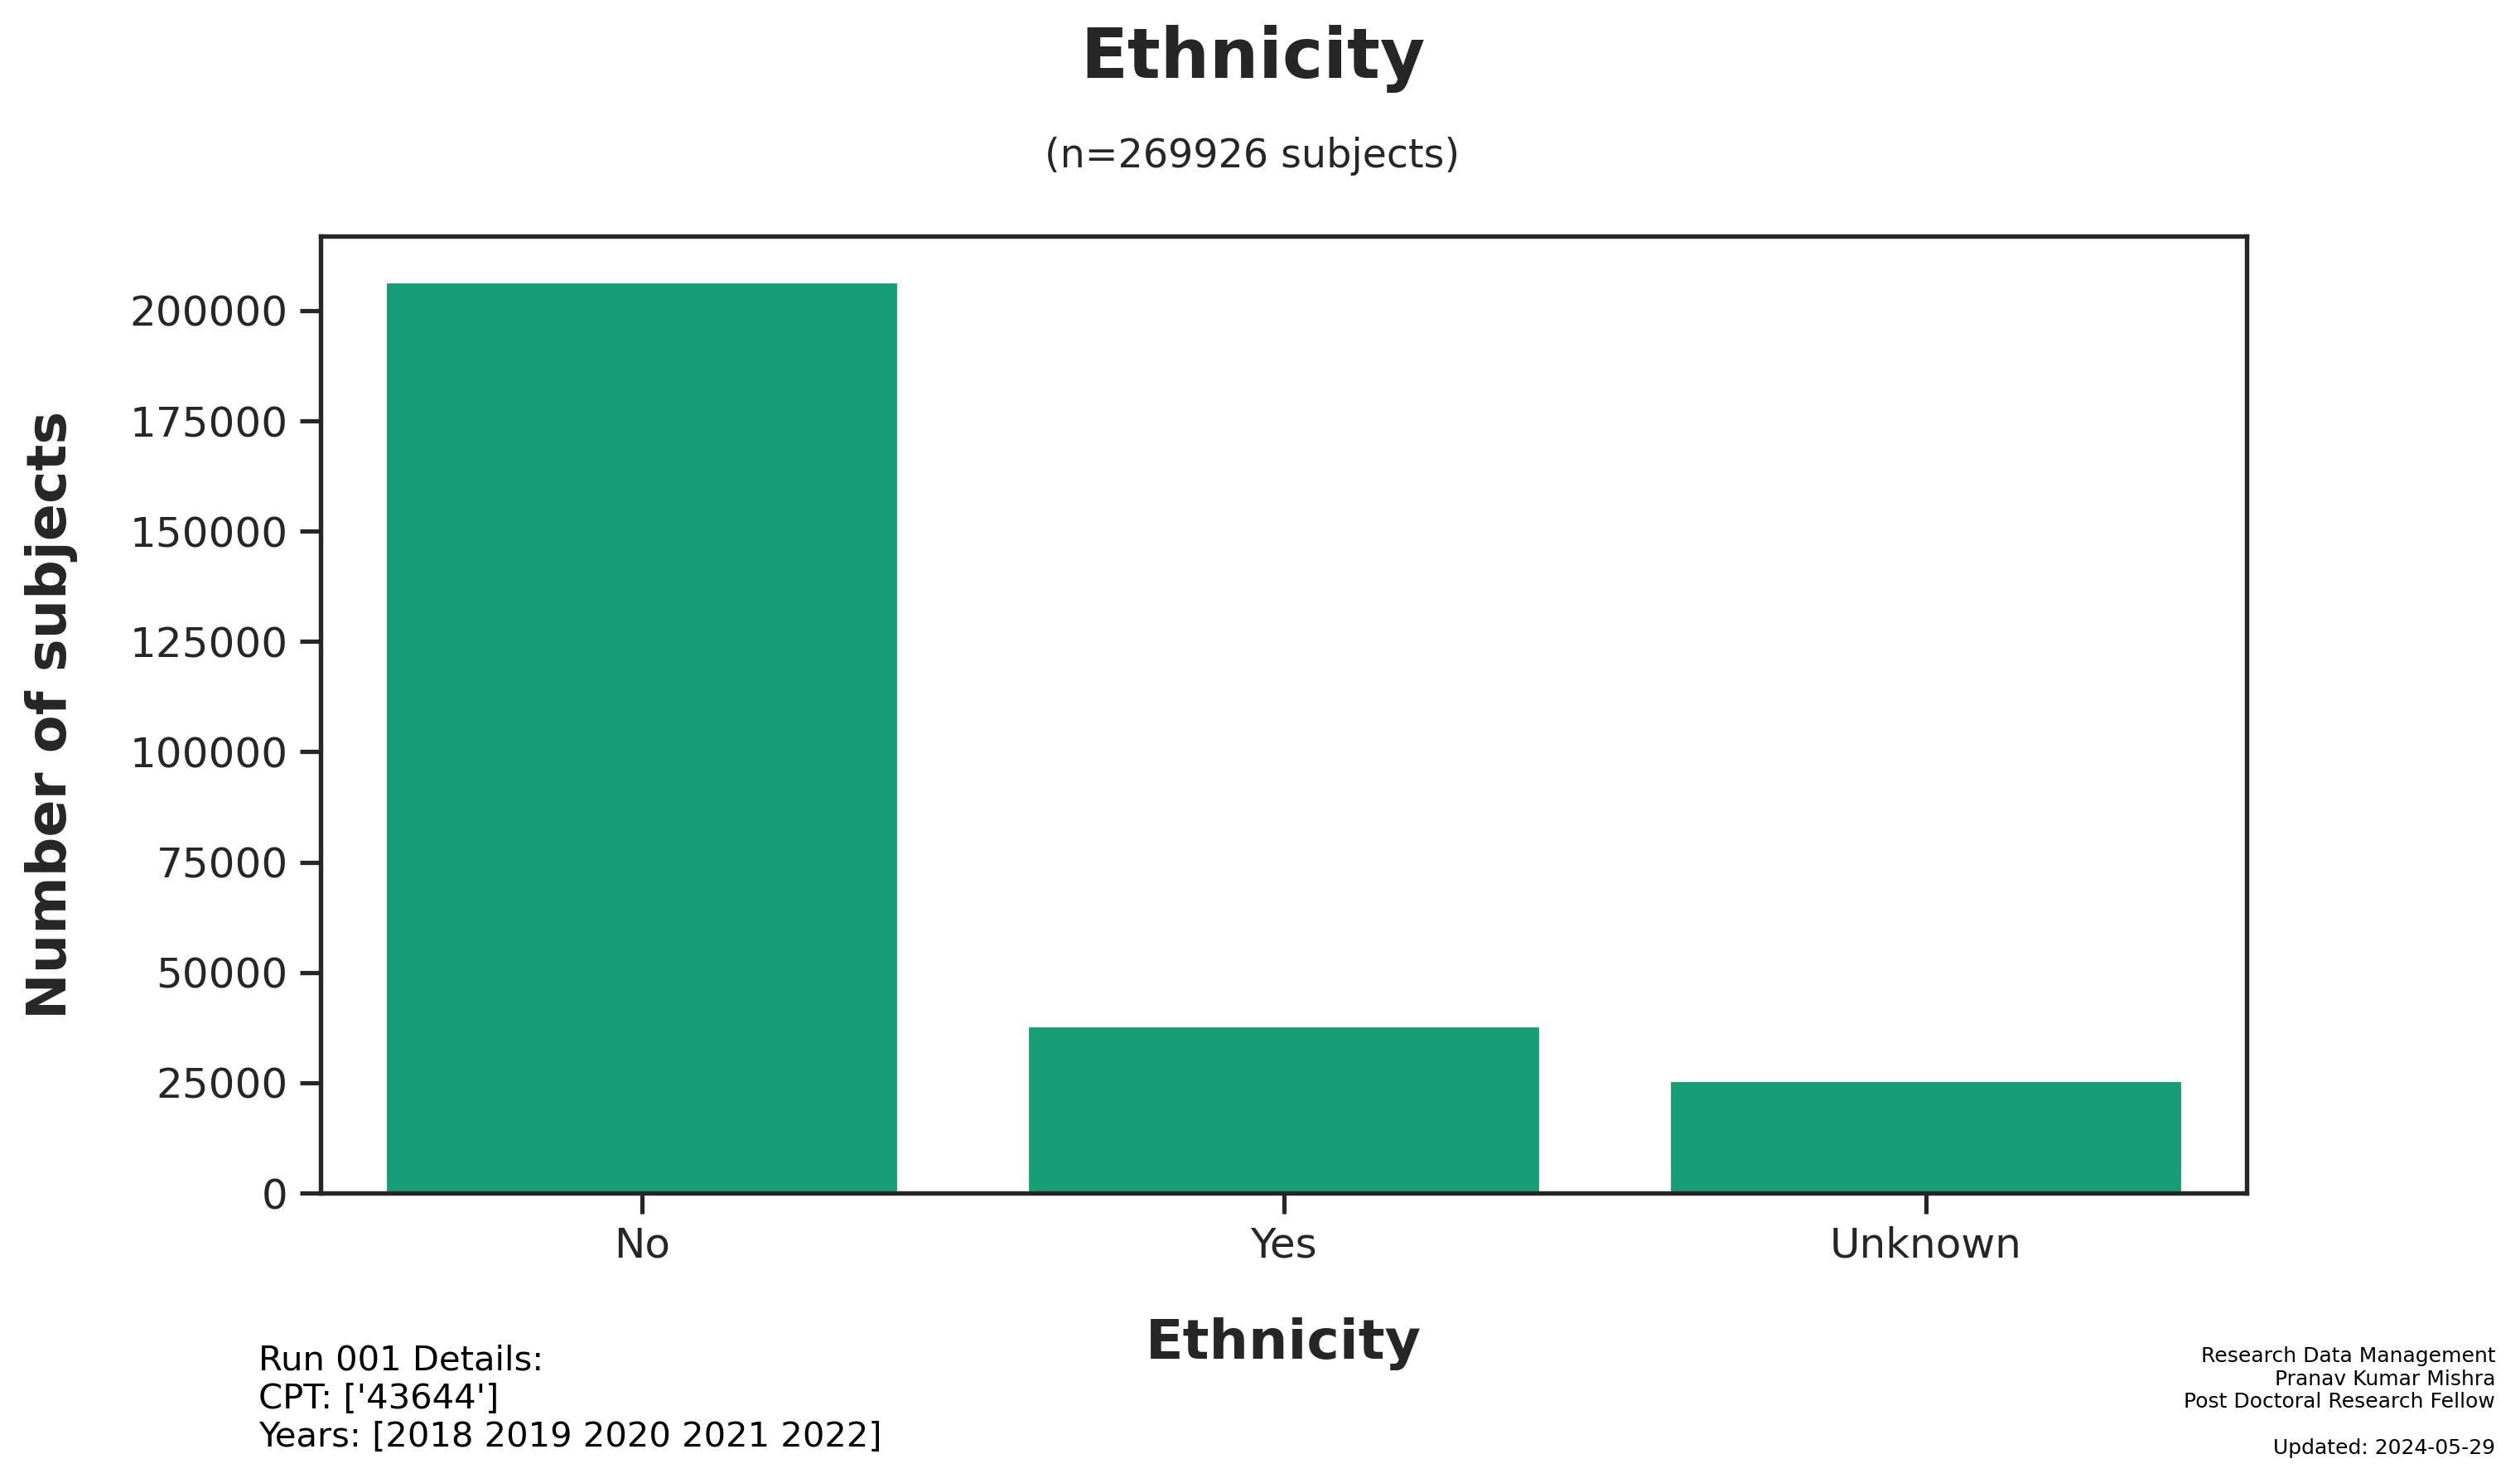
\includegraphics{figures/demographics/Run001_Demographics-Ethnicity.jpg}

}

\caption{Run001\_Demographics-Ethnicity.jpg}

\end{figure}%%
\begin{figure}[H]

{\centering 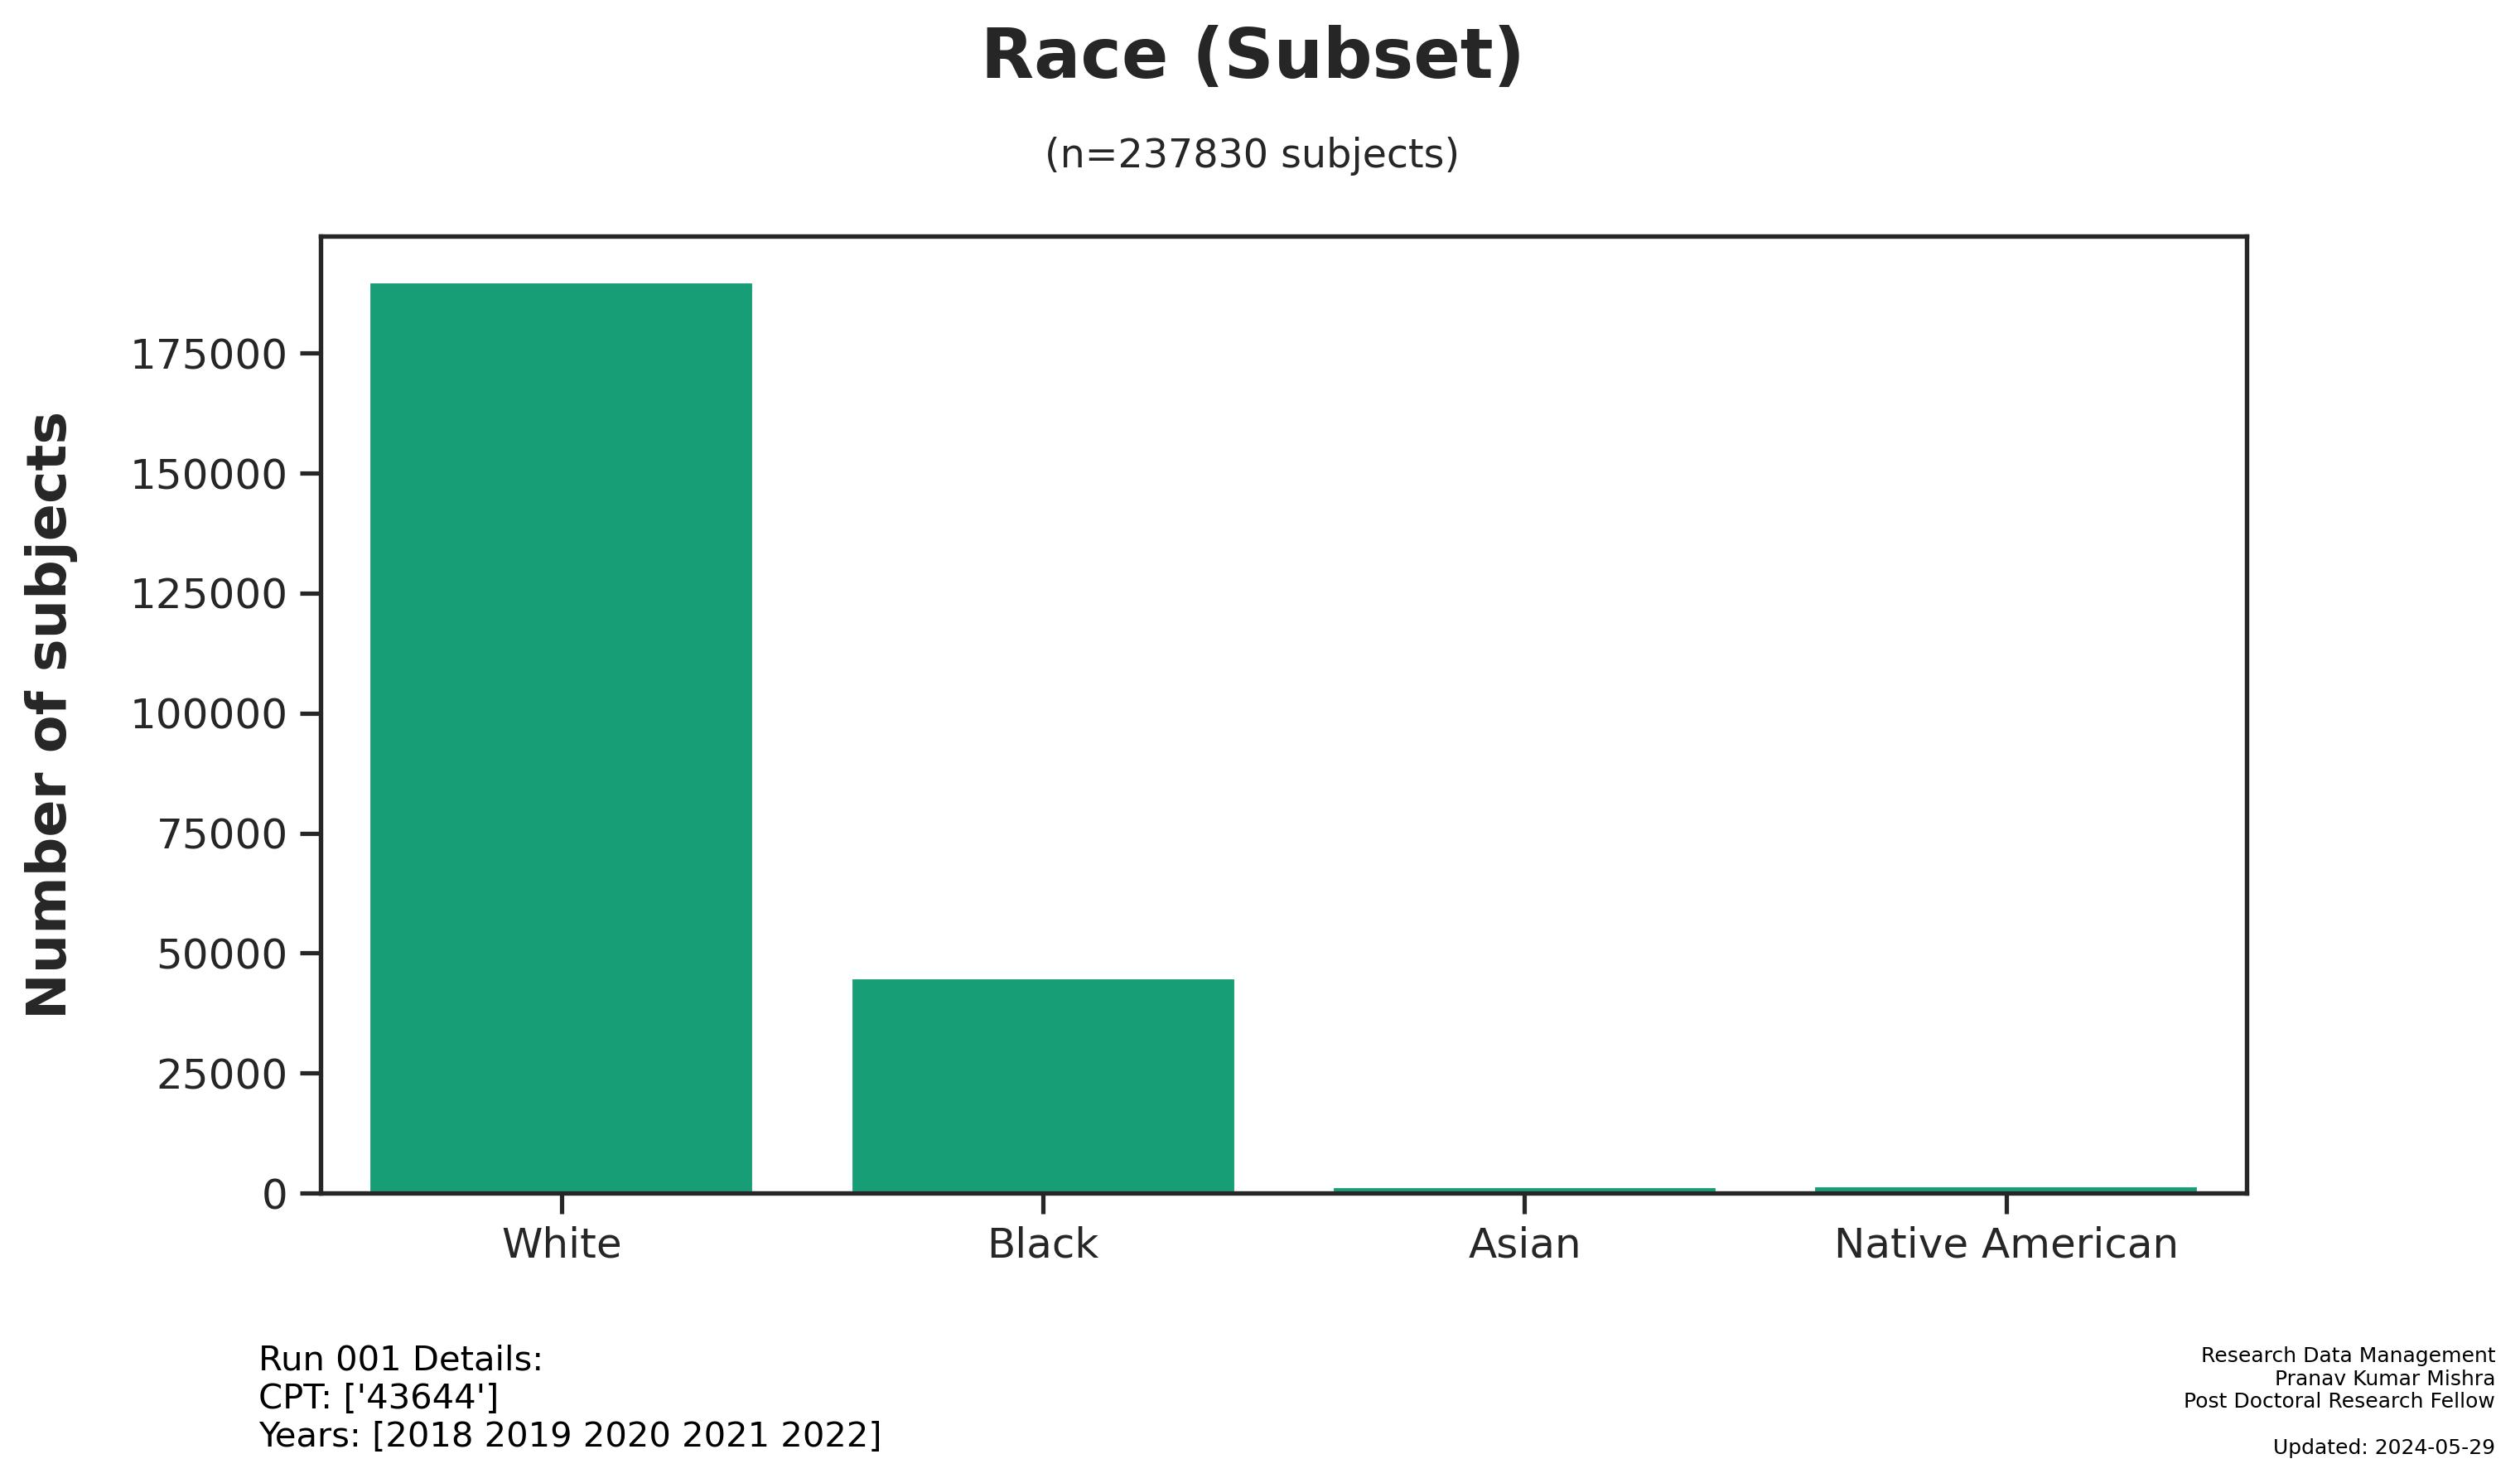
\includegraphics{figures/demographics/Run001_Demographics-Race.jpg}

}

\caption{Run001\_Demographics-Race.jpg}

\end{figure}%%
\begin{figure}[H]

{\centering 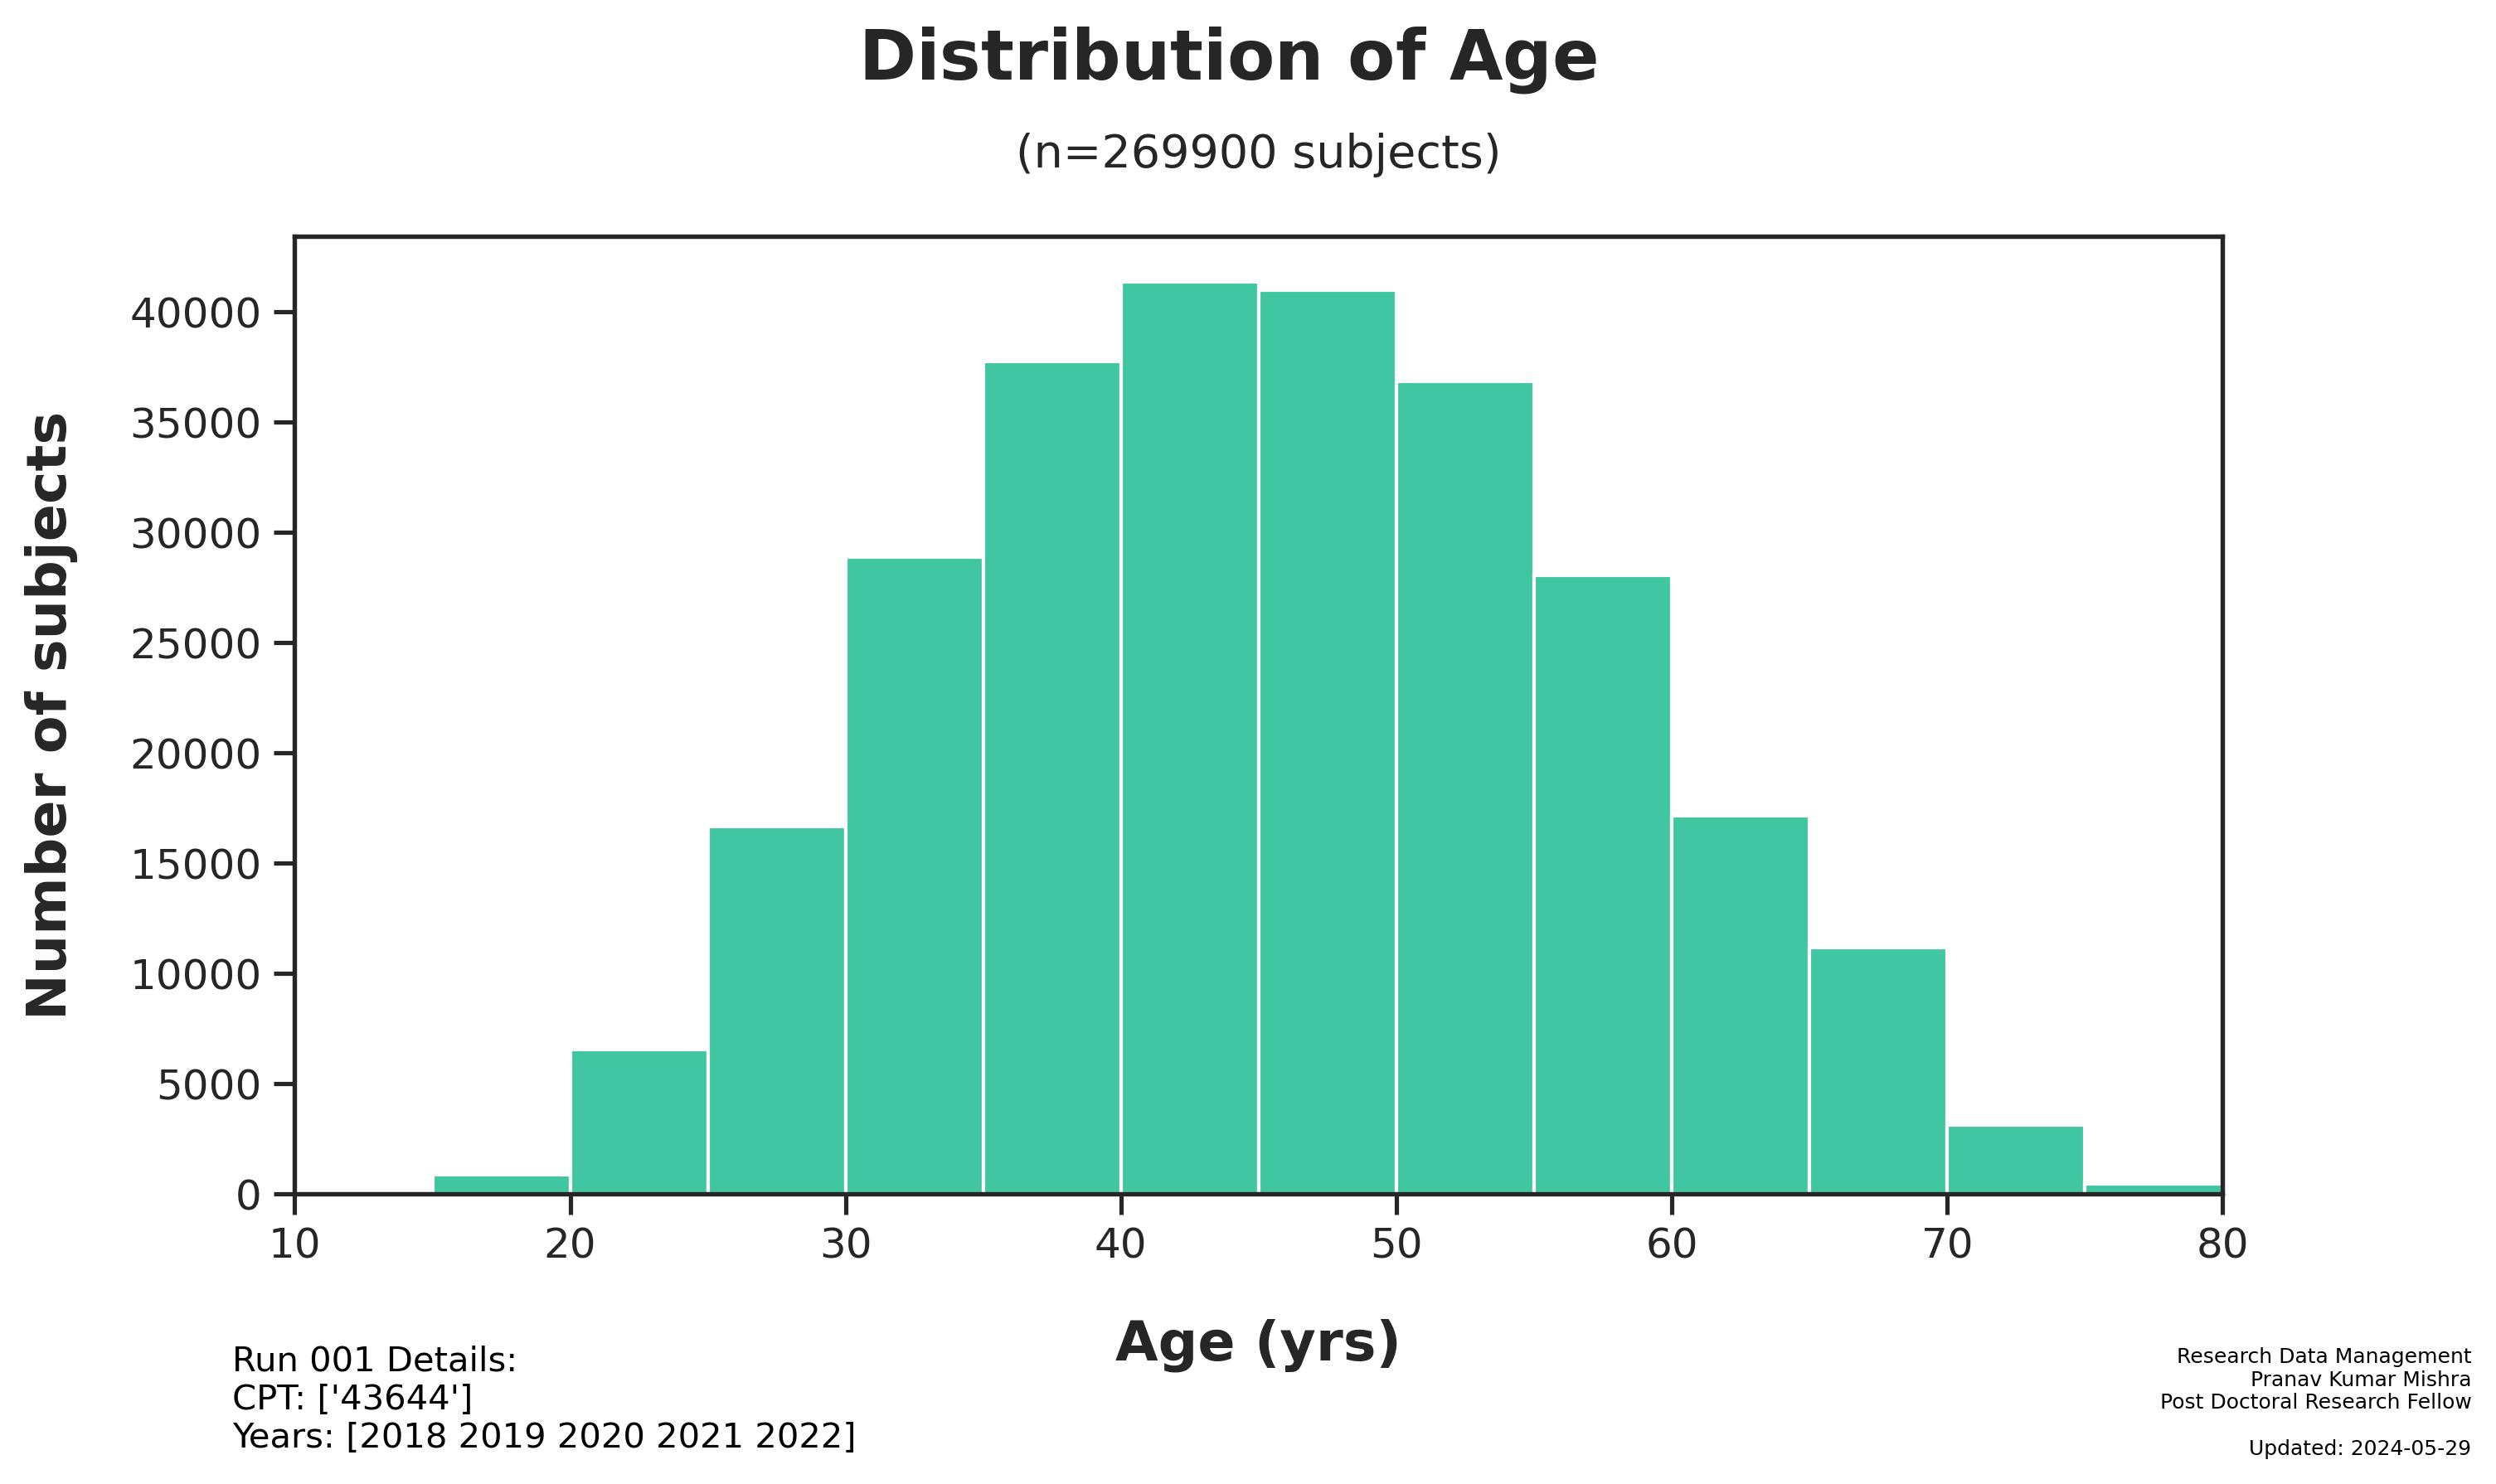
\includegraphics{figures/demographics/Run001_Demographics_Age_at_Surgery.jpg}

}

\caption{Run001\_Demographics\_Age\_at\_Surgery.jpg}

\end{figure}%%
\begin{figure}[H]

{\centering 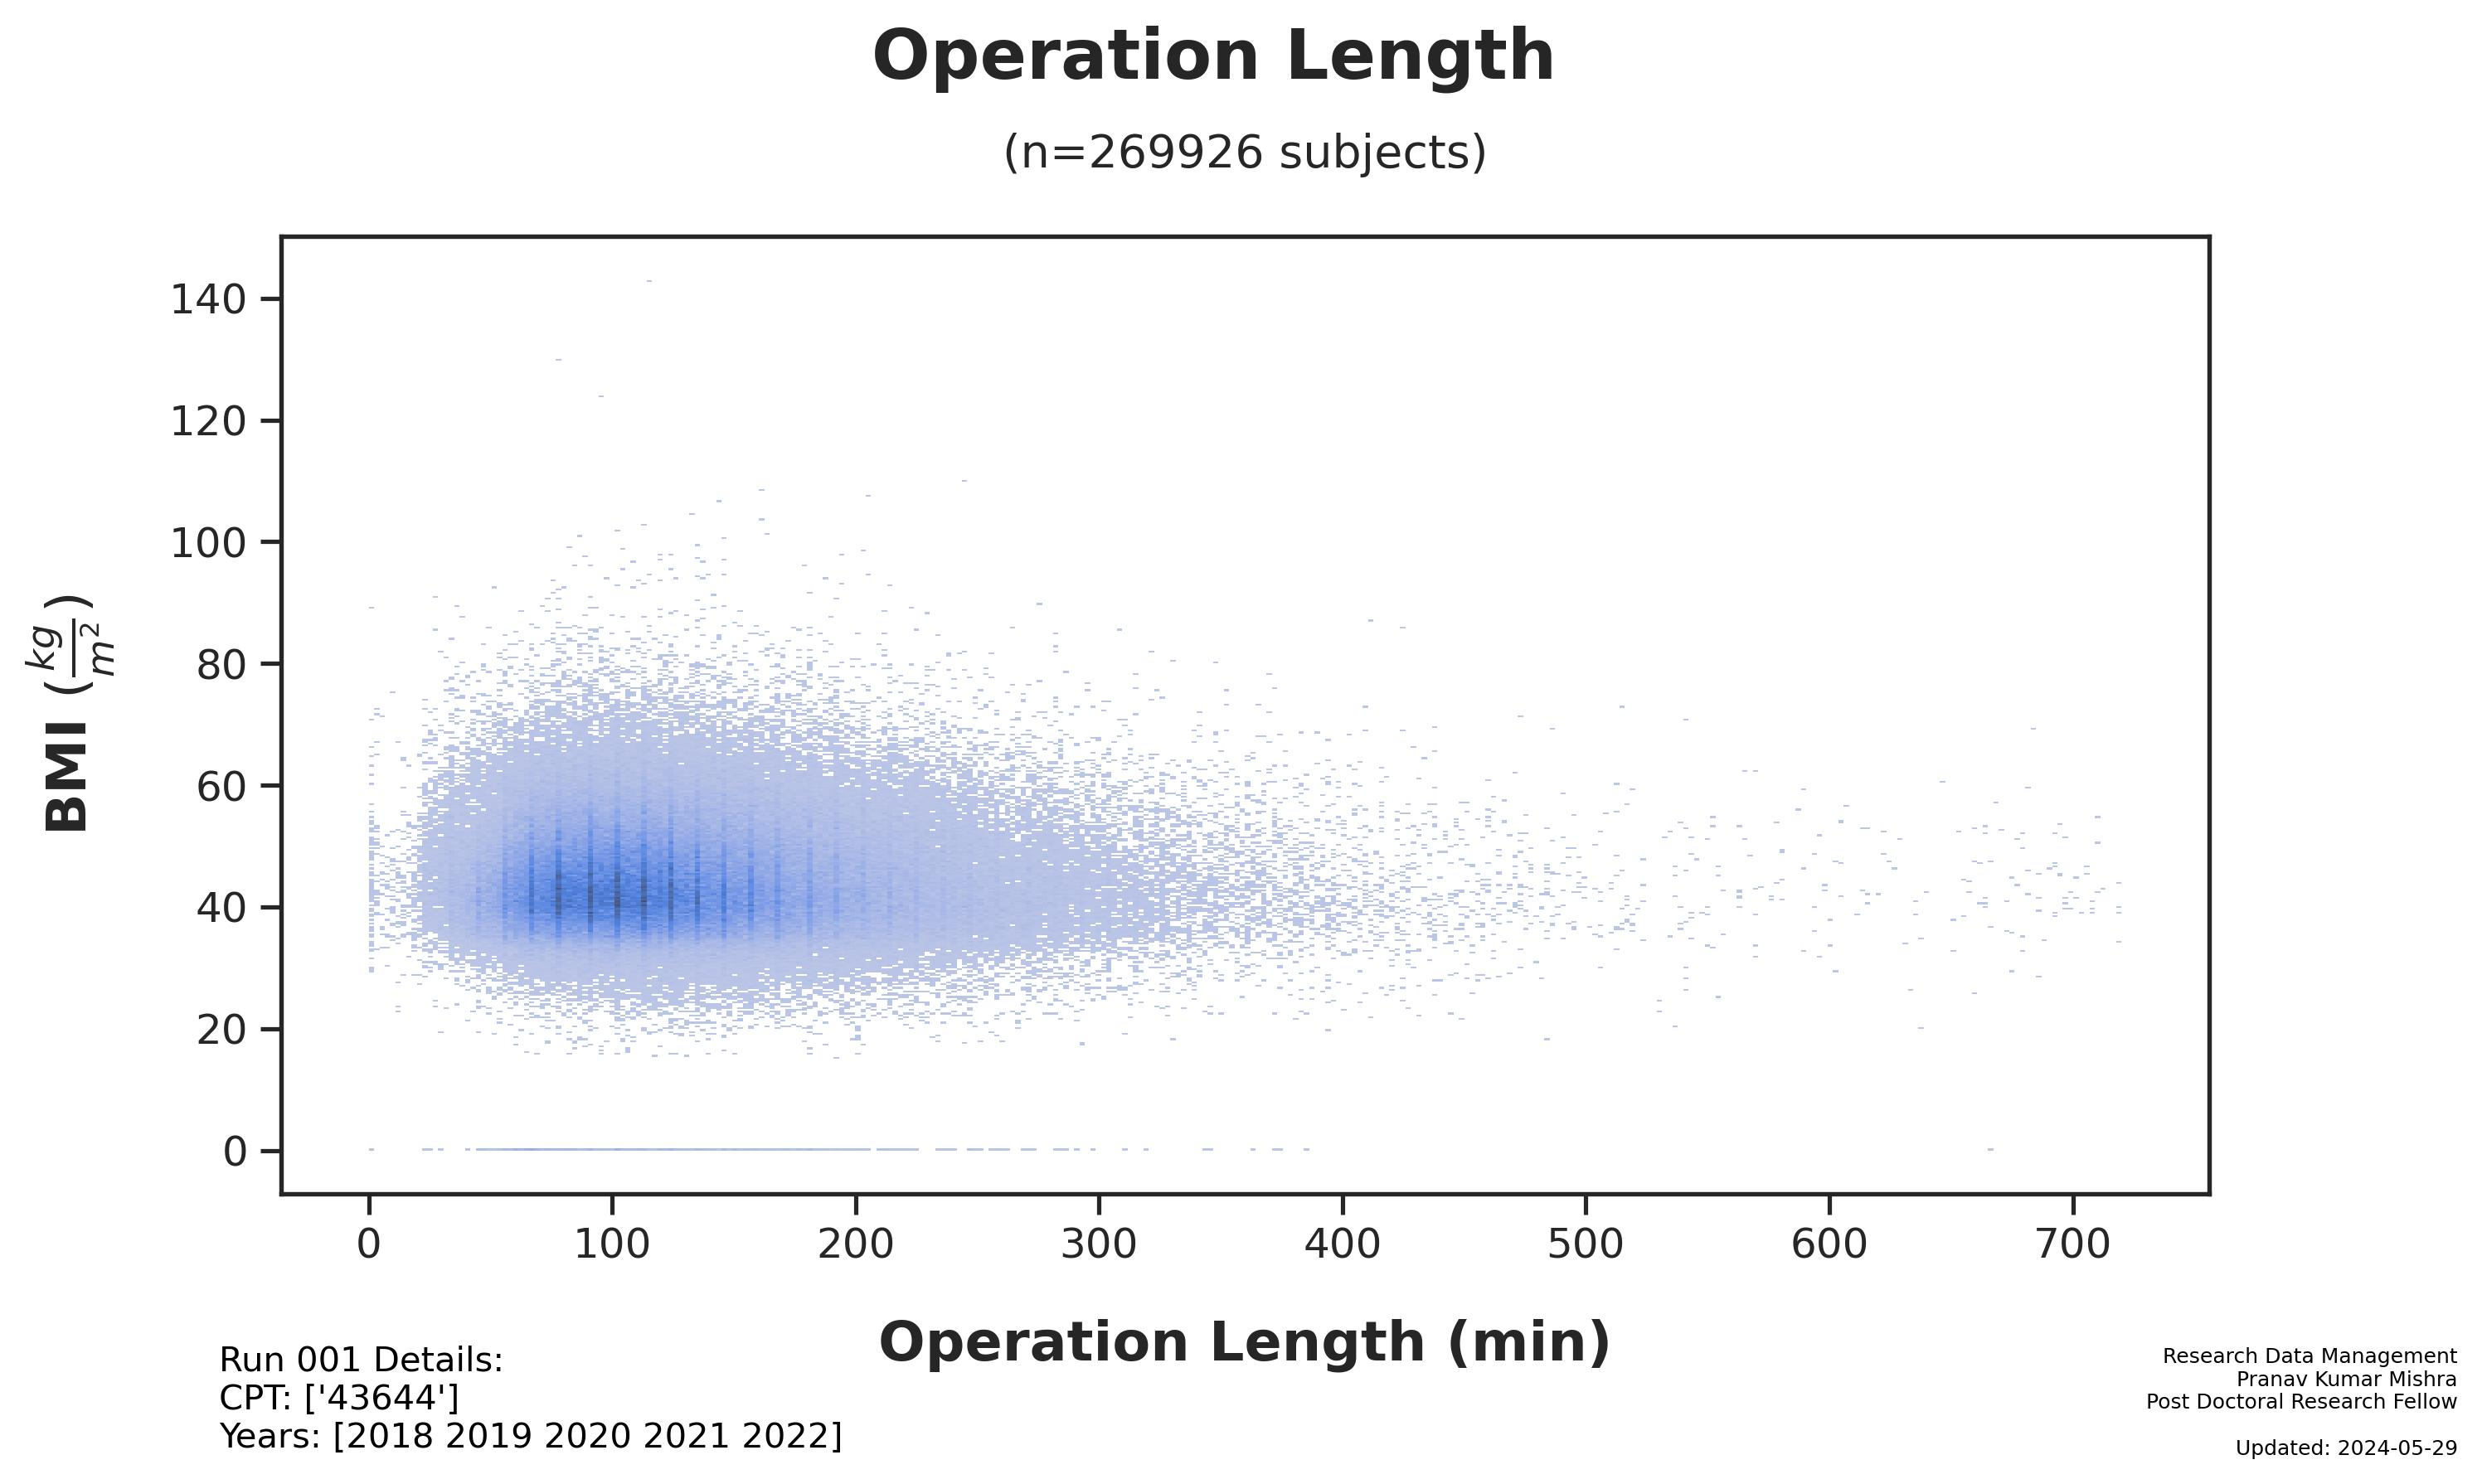
\includegraphics{figures/surgery/Run001_Sx-OPLENGTH_PREVSURG.jpg}

}

\caption{Run001\_Sx-OPLENGTH\_PREVSURG.jpg}

\end{figure}%%
\begin{figure}[H]

{\centering \includegraphics{notebooks/Run001_analysis_files/figure-html/cell-14-output-1.png}

}

\caption{cell-14-output-1.png}

\end{figure}%%
\begin{figure}[H]

{\centering \includegraphics{notebooks/Run001_analysis_files/figure-html/cell-15-output-2.png}

}

\caption{cell-15-output-2.png}

\end{figure}%%
\begin{figure}[H]

{\centering \includegraphics{notebooks/Run001_analysis_files/figure-html/cell-16-output-2.png}

}

\caption{cell-16-output-2.png}

\end{figure}%%
\begin{figure}[H]

{\centering \includegraphics{notebooks/Run001_analysis_files/figure-html/cell-17-output-2.png}

}

\caption{cell-17-output-2.png}

\end{figure}%%
\begin{figure}[H]

{\centering \includegraphics{notebooks/Run001_analysis_files/figure-html/cell-18-output-2.png}

}

\caption{cell-18-output-2.png}

\end{figure}%%
\begin{figure}[H]

{\centering \includegraphics{notebooks/Run001_analysis_files/figure-pdf/cell-14-output-1.png}

}

\caption{cell-14-output-1.png}

\end{figure}%%
\begin{figure}[H]

{\centering \includegraphics{notebooks/Run001_analysis_files/figure-pdf/cell-15-output-2.png}

}

\caption{cell-15-output-2.png}

\end{figure}%%
\begin{figure}[H]

{\centering \includegraphics{notebooks/Run001_analysis_files/figure-pdf/cell-16-output-2.png}

}

\caption{cell-16-output-2.png}

\end{figure}%%
\begin{figure}[H]

{\centering \includegraphics{notebooks/Run001_analysis_files/figure-pdf/cell-17-output-2.png}

}

\caption{cell-17-output-2.png}

\end{figure}%%
\begin{figure}[H]

{\centering \includegraphics{notebooks/Run001_analysis_files/figure-pdf/cell-18-output-2.png}

}

\caption{cell-18-output-2.png}

\end{figure}%

\subsection{Files}\label{files}

The following files were generated from Run 001:

\begin{itemize}
\tightlist
\item
  readme.md
\item
  readme.html
\item
  readme-gfm.md
\item
  readme.pdf
\item
  figures/demographics/Run001\_Demographics-Donor\_Sex.jpg
\item
  figures/demographics/Run001\_Demographics-Ethnicity.jpg
\item
  figures/demographics/Run001\_Demographics-Race.jpg
\item
  figures/demographics/Run001\_Demographics\_Age\_at\_Surgery.jpg
\item
  figures/surgery/Run001\_Sx-OPLENGTH\_PREVSURG.jpg
\item
  notebooks/Run001\_analysis.ipynb
\item
  notebooks/Run001\_analysis.html
\item
  notebooks/Run001\_analysis.tex
\item
  notebooks/Run001\_analysis.aux
\item
  notebooks/Run001\_analysis.toc
\item
  notebooks/Run001\_analysis.log
\item
  notebooks/Run001\_analysis\_files/figure-html/cell-14-output-1.png
\item
  notebooks/Run001\_analysis\_files/figure-html/cell-15-output-2.png
\item
  notebooks/Run001\_analysis\_files/figure-html/cell-16-output-2.png
\item
  notebooks/Run001\_analysis\_files/figure-html/cell-17-output-2.png
\item
  notebooks/Run001\_analysis\_files/figure-html/cell-18-output-2.png
\item
  notebooks/Run001\_analysis\_files/figure-pdf/cell-14-output-1.png
\item
  notebooks/Run001\_analysis\_files/figure-pdf/cell-15-output-2.png
\item
  notebooks/Run001\_analysis\_files/figure-pdf/cell-16-output-2.png
\item
  notebooks/Run001\_analysis\_files/figure-pdf/cell-17-output-2.png
\item
  notebooks/Run001\_analysis\_files/figure-pdf/cell-18-output-2.png
\item
  tables/Run001\_demo\_selected.csv
\item
  tables/Run001\_main\_dataset.parquet
\end{itemize}



\end{document}
